\documentclass[14pt]{beamer}

\usepackage{xcolor}
\usepackage{colortbl}
\usepackage{pgf}
\usepackage{amsmath}
\usepackage{amssymb}
\usepackage{latexsym}
\usepackage{tikz}
\usepackage{pgfplots}
\usepackage{pdfpages}
\usepackage{ulem}

\definecolor{shaded}{RGB}{210,210,210}
\usecolortheme[named=shaded]{structure}

\definecolor{stressed}{RGB}{150,40,40}
\setbeamercolor{alerted_text}{fg=stressed}


\setbeamertemplate{navigation symbols}{}
\setbeamersize{text margin left=3mm} 
\setbeamersize{text margin right=3mm} 

%\usepackage{fontspec,xunicode,xltxtra}
%\setmainfont{Helvetica Neue Light}
%\setsansfont{Helvetica Neue Light}

%\usepackage[T1]{fontenc}
%\usepackage{tgheros}
%\renewcommand*\familydefault{\sfdefault} %% Only if the base font of the document is to be sans serif

\setbeamertemplate{sidebar right}{default}{}

\makeatletter
\define@key{beamerframe}{nofills}[true]{% top
  \beamer@frametopskip=0pt\relax%
  \beamer@framebottomskip=0pt\relax%
  \beamer@frametopskipautobreak=\beamer@frametopskip\relax%
  \beamer@framebottomskipautobreak=\beamer@framebottomskip\relax%
  \def\beamer@initfirstlineunskip{%
    \def\beamer@firstlineitemizeunskip{%
      \vskip-\partopsep\vskip-\topsep\vskip-\parskip%
      \global\let\beamer@firstlineitemizeunskip=\relax}%
    \everypar{\global\let\beamer@firstlineitemizeunskip=\relax}}
}
\makeatother

\newcommand{\setbackgroundpicturewhite}[1]{%
\usebackgroundtemplate{%
\begin{tikzpicture}%
\draw[fill=white] (current page.north west) rectangle (current page.south east);%
\node[draw,minimum width=\paperwidth,minimum height=\paperheight] [anchor=south west] (mynode) {\includegraphics[width=\paperwidth]{#1}};%
\end{tikzpicture}%
}%
%\begin{pgfpicture}{0in}{0in}{\paperwidth}{\paperheight}
%\pgfputat{\pgfxy(0,0)}{\includegraphics[width=\paperwidth]{#1}}
%\color{white}
%\pgfsetfillopacity{0.0}
%\pgfrect[fill]{\pgfxy(0,0)}{\pgfpoint{\paperwidth}{\paperheight}}
%\end{pgfpicture}
%}
}


\newcommand{\setbackgroundpictureblack}[1]{%
\usebackgroundtemplate{%
\begin{tikzpicture}%
\draw[fill=black] (current page.north west) rectangle (current page.south east);%
\node[draw,minimum width=\paperwidth,minimum height=\paperheight] [anchor=south west] (mynode) {\includegraphics[width=\paperwidth]{#1}};%
\end{tikzpicture}%
}%
%\begin{pgfpicture}{0in}{0in}{\paperwidth}{\paperheight}
%\pgfputat{\pgfxy(0,0)}{\includegraphics[width=\paperwidth]{#1}}
%\color{white}
%\pgfsetfillopacity{0.0}
%\pgfrect[fill]{\pgfxy(0,0)}{\pgfpoint{\paperwidth}{\paperheight}}
%\end{pgfpicture}
%}
}


\newcommand{\setdarkbackgroundpictureblack}[1]{%
\usebackgroundtemplate{%
\begin{tikzpicture}%
\draw[fill=black] (current page.north west) rectangle (current page.south east);%
\node[draw,very thick,minimum width=\paperwidth-\pgflinewidth,minimum height=\paperheight-\pgflinewidth] [anchor=south west] (mynode) {\includegraphics[width=\paperwidth]{#1}};%
\draw[fill=black,opacity=0.75] (current page.north west) rectangle (current page.south east);%
\end{tikzpicture}%
}}%


\newcommand{\setdarkbackgroundpicturewhite}[1]{%
\usebackgroundtemplate{%
\begin{tikzpicture}%
\draw[fill=white] (current page.north west) rectangle (current page.south east);%
\node[draw,very thick,minimum width=\paperwidth-\pgflinewidth,minimum height=\paperheight-\pgflinewidth] [anchor=south west] (mynode) {\includegraphics[width=\paperwidth]{#1}};%
\draw[fill=white,opacity=0.75] (current page.north west) rectangle (current page.south east);%
\end{tikzpicture}%
}}%


\newcommand{\clearbackgroundpicture}{\usebackgroundtemplate{}}

\begin{document}
\setbeamercolor{background canvas}{bg=white,fg=black}
\usebeamercolor[fg]{background canvas}

%%%%%%%%%%%%%%%%%%%%%%%%%%%%%%%%%%%%%%%%%%%%%%%%%%%%%%%%%%%%%%%%
\clearbackgroundpicture
\begin{frame}[nofills]
  
\includegraphics[width=\textwidth]{cow.pdf}

  \vfill
  \Large
  \textsf{\textbf{Jim Fowler, Steve Gubkin,}} \\
  \textsf{\textbf{David Lindberg, Bart Snapp}} \\
  \textsf{OSU Mathematics Department}
\end{frame}

\begin{frame}
  \Huge \textbf{MOOC\only<1>{?}\only<2>{ $=$}}

  \vfill

  \uncover<2->{
  \textbf{M}assive \\
  \textbf{O}pen \\
  \textbf{O}nline \\
  \textbf{C}ourse \\
  }

  \vfill
\end{frame}

%%%%%%%%%%%%%%%%%%%%%%%%%%%%%%%%%%%%%%%%%%%%%%%%%%%%%%%%%%%%%%%%
% Coursera
\setbackgroundpicturewhite{calculus-one-landing.png}
\begin{frame}
\end{frame}

\setdarkbackgroundpicturewhite{calculus-one-landing.png}
\begin{frame}
\huge\textsf{\textbf{85k enrollments}}
\end{frame}

\begin{frame}
  \vfill
  \only<1>{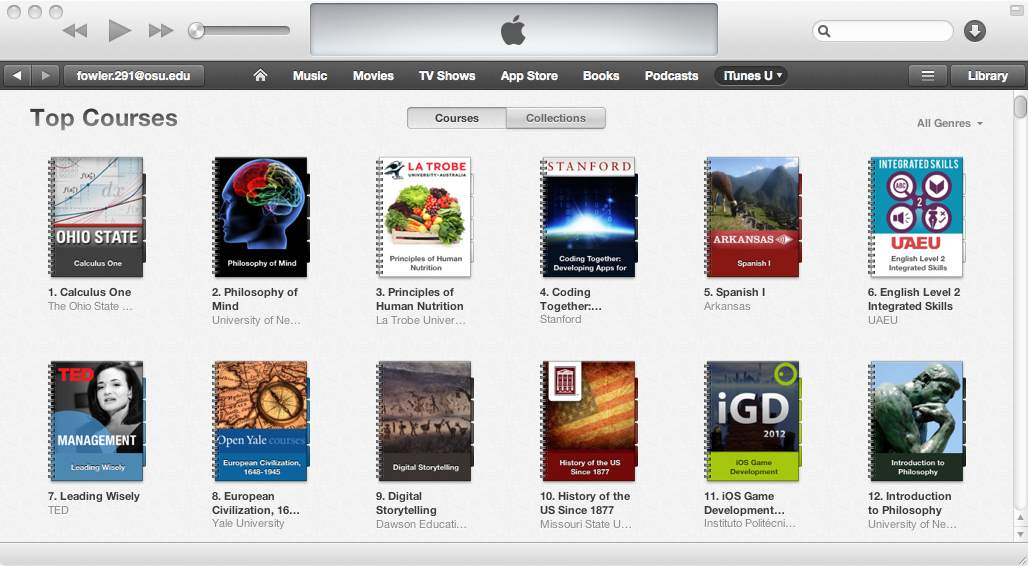
\includegraphics[width=\textwidth]{number-one.jpg}}
  \only<2-3>{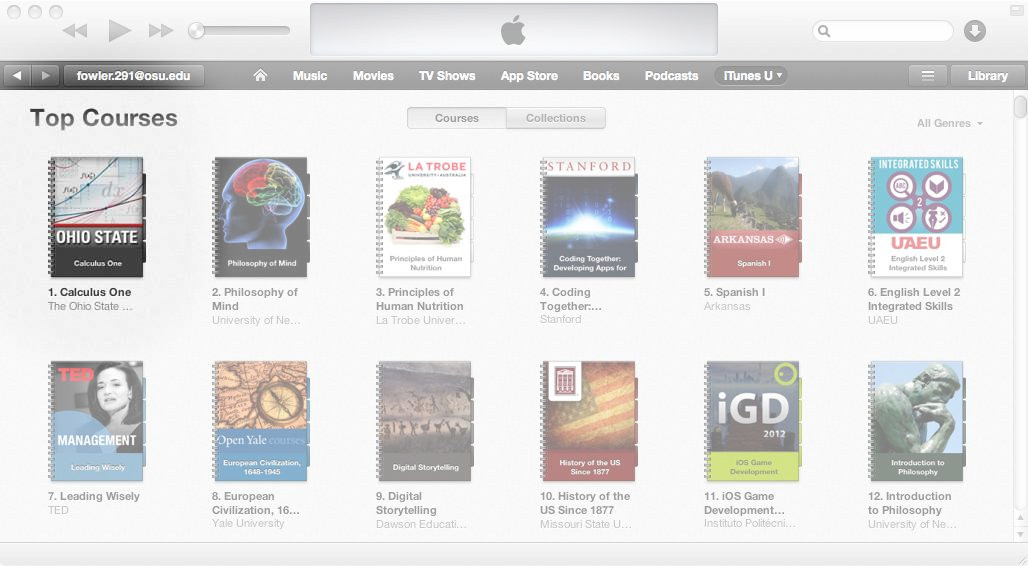
\includegraphics[width=\textwidth]{number-one-highlight.jpg}}

  \uncover<3>{\begin{center}\Large\textbf{37k subscribed on iTunes U}\end{center}}
  \vfill
\end{frame}

\clearbackgroundpicture
\begin{frame}[nofills]
  \vfill
  \scalebox{3}{\textsf{Who are}} \\
  \scalebox{3}{\textsf{these students?}}
  \vfill
\end{frame}

\setbackgroundpicturewhite{sequences-landing.png}
\begin{frame}
\end{frame}

\setdarkbackgroundpicturewhite{sequences-landing.png}
\begin{frame}[nofills]
\vfill
\huge\textsf{\textbf{Starts\ldots tomorrow!}}
\vfill
\end{frame}

\setbackgroundpictureblack{coursera-video.jpg}
\begin{frame}
\end{frame}

\setbackgroundpicturewhite{mooculus-textbook-page.pdf}
\begin{frame}[nofills]
\end{frame}


\usebackgroundtemplate{
\includegraphics[height=\paperheight]{blackboard.png}}
\begin{frame}
\begin{center}
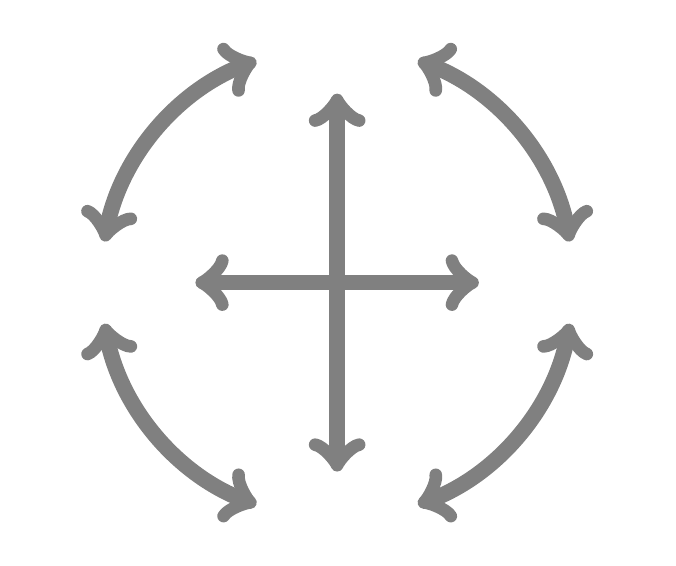
\begin{tikzpicture}[scale=3]
%\draw[help lines] (0,0) grid (5,4);
\draw [gray,<->,line width=2mm] (.342,.940) arc [radius=1, start angle=70, end angle =10];
\draw [gray,<->,line width=2mm] (.985,-.174) arc [radius=1, start angle=-10, end angle =-70];
\draw [gray,<->,line width=2mm] (-.342,-.940) arc [radius=1, start angle=250, end angle =190];
\draw [gray,<->,line width=2mm] (-.9850,.174) arc [radius=1, start angle=170, end angle =110];

\draw [gray,<->,line width=2mm] (-.6,0)--(.6,0);
\draw [gray,<->,line width=2mm] (0,.8)--(0,-.8);


\node at (0,1) [white] {\textbf{Lectures}};
\node at (1,0) [white] {\textbf{Textbook}};
\node at (-1,0) [white] {\textbf{Exercises}};
\node at (0,-1) [white] {\textbf{Forum}};
\end{tikzpicture}
\end{center}
\end{frame}

\setbackgroundpicturewhite{coursera-quiz.png}
\begin{frame}
\end{frame}

\setdarkbackgroundpicturewhite{coursera-quiz.png}
\begin{frame}
\huge\textsf{\textbf{Ten questions per quiz.}}

%\vspace{1cm}\pause

%\huge\textsf{It's a paper quiz, but online.}
\end{frame}

\begin{frame}[nofills]
  \vfill
  \huge\textsf{How many questions \textit{should} \\
\quad be on a quiz?}
 \vfill\pause
  \huge\textsf{\textbf{Depends on the student!}}
\vfill
\end{frame}

%%%%%%%%%%%%%%%%%%%%%%%%%%%%%%%%%%%%%%%%%%%%%%%%%%%%%%%%%%%%%%%%
% Mooculus
\setbackgroundpictureblack{mooculus-landing-page.png}
\begin{frame}
\end{frame}

%%%%%%%%%%%%%%%%%%%%%%%%%%%%%%%%%%%%%%%%%%%%%%%%%%%%%%%%%%%%%%%%
\clearbackgroundpicture
\begin{frame}[nofills]
  \vfill
  \scalebox{3}{\textsf{What is}}
  
\includegraphics[width=0.8\textwidth]{cow.pdf}\raisebox{0.25in}{\scalebox{5}{?}}
  \vfill
  \pause
  \huge{Online homework, \pause with \\\quad a hidden Markov model.}
  \vfill
\end{frame}

%%%%%%%%%%%%%%%%%%%%%%%%%%%%%%%%%%%%%%%%%%%%%%%%%%%%%%%%%%%%%%%%
% Mooculus as an exercise platform
\setbackgroundpictureblack{mooculus-exercise-1.png}
\begin{frame}
\end{frame}
\setbackgroundpictureblack{mooculus-exercise-1-highlight.png}
\begin{frame}[nofills]
\pause
\vfill
\vspace{1.5cm}
\huge\color{red!75!black}
We've built a \\
\quad computer algebra \\
\quad\quad system \\
\quad in JavaScript.
\vfill
\end{frame}
\setbackgroundpictureblack{mooculus-exercise-1.png}
\begin{frame}
\end{frame}
\setbackgroundpictureblack{mooculus-exercise-hint.png}
\begin{frame}
\end{frame}
\setbackgroundpictureblack{mooculus-exercise-1.png}
\begin{frame}
\end{frame}
\setbackgroundpictureblack{mooculus-exercise-2.png}
\begin{frame}
\end{frame}
\setbackgroundpictureblack{mooculus-exercise-3.png}
\begin{frame}
\end{frame}
\setbackgroundpictureblack{mooculus-exercise-4.png}
\begin{frame}
\end{frame}
\setbackgroundpictureblack{mooculus-exercise-5.png}
\begin{frame}
\end{frame}
\setbackgroundpictureblack{mooculus-exercise-progress.png}
\begin{frame}
\end{frame}

\setbackgroundpictureblack{mooculus-exercise-progress.png}
\begin{frame}[nofills]
\vfill\vfill
\Huge
Student understanding\\
\quad is invisible.
\vfill\pause
Hints and answers \\
\quad are visible.
\vfill
\vfill
\end{frame}

\setbackgroundpictureblack{mooculus-exercise-index.png}
\begin{frame}
\end{frame}

\clearbackgroundpicture
\begin{frame}[nofills]
\Huge\textbf{What's the benefit?}

\vfill
\uncover<2->{\hfill\alt<1-2>{Cheaper?}{\textcolor{gray}{\sout{Cheaper?}}}%
\hfill\uncover<3->{\textcolor{red!50!black}{Better!}}\hfill\null}
\vfill
 
\end{frame}

\setbackgroundpictureblack{Math_lecture_at_TKK.jpg}
\begin{frame}
\end{frame}

\setdarkbackgroundpictureblack{Math_lecture_at_TKK.jpg}
\begin{frame}[nofills]
\vfill
\Huge\color{white}
Doing mathematics \\
\vfill
\quad is better than \\
\vfill
watching mathematics.
\vfill
\end{frame}

%%% SEGUE: So this cheaper versus better dichotomy is one misunderstanding
%%% about MOOCs; here's another

\clearbackgroundpicture
\begin{frame}[nofills]
\Huge\textbf{What's \textit{massive}?}

\vfill
\uncover<2->{\hfill\alt<1-2>{Enrollment?}{\textcolor{gray}{\sout{Enrollment?}}}%
\hfill\uncover<3->{\textcolor{red!50!black}{Data!}}\hfill\null}
\vfill
 
\end{frame}

\begin{frame}[nofills]
\huge
\vfill
10.3 person--years
\vfill
2,079,428 correct answers
\vfill
\end{frame}

\begin{frame}[nofills]
\begin{center}
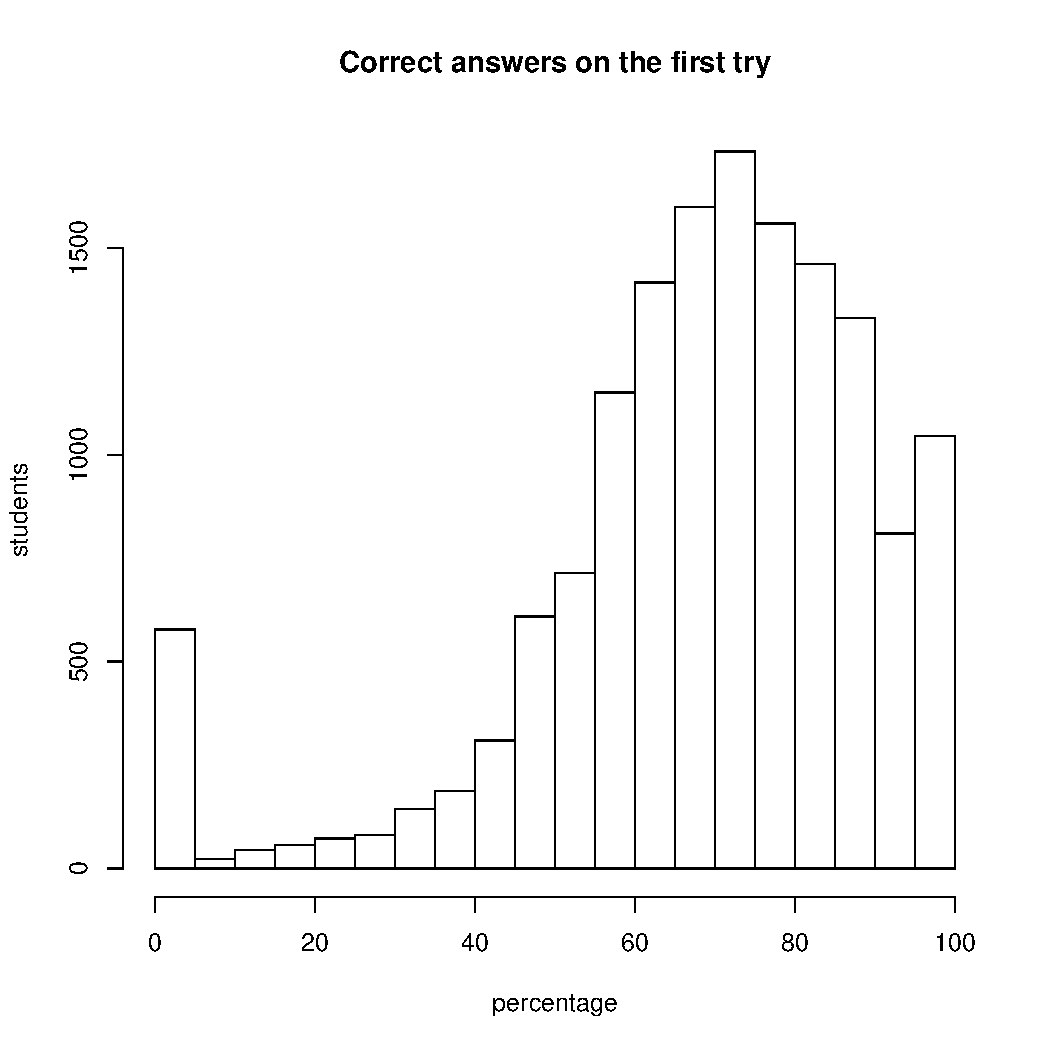
\includegraphics[height=0.9\textheight]{histogram-student-aces.pdf}
\end{center}
\end{frame}

\begin{frame}[nofills]
\begin{center}
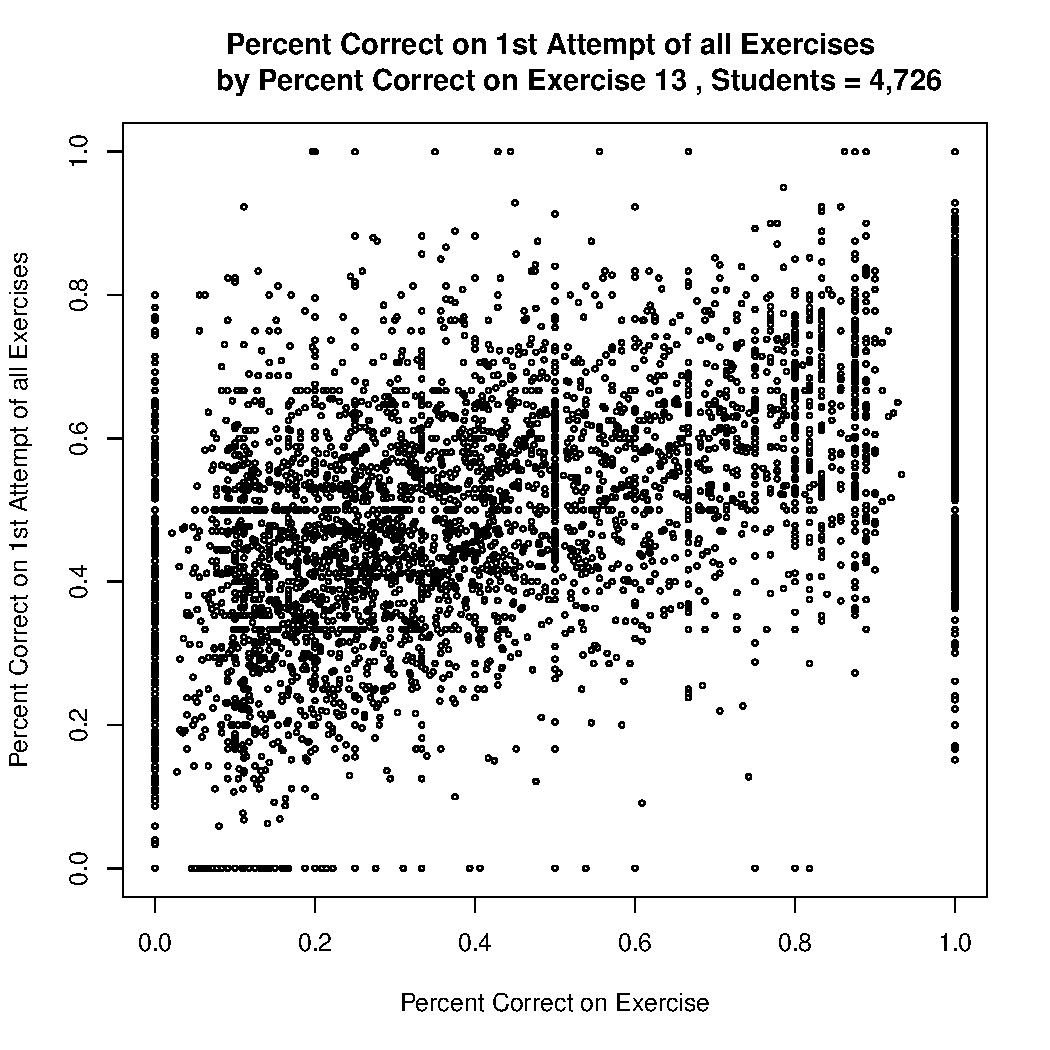
\includegraphics[height=0.9\textheight]{exercise-odds-13.pdf}
\end{center}
\end{frame}

\begin{frame}[nofills]
\begin{center}
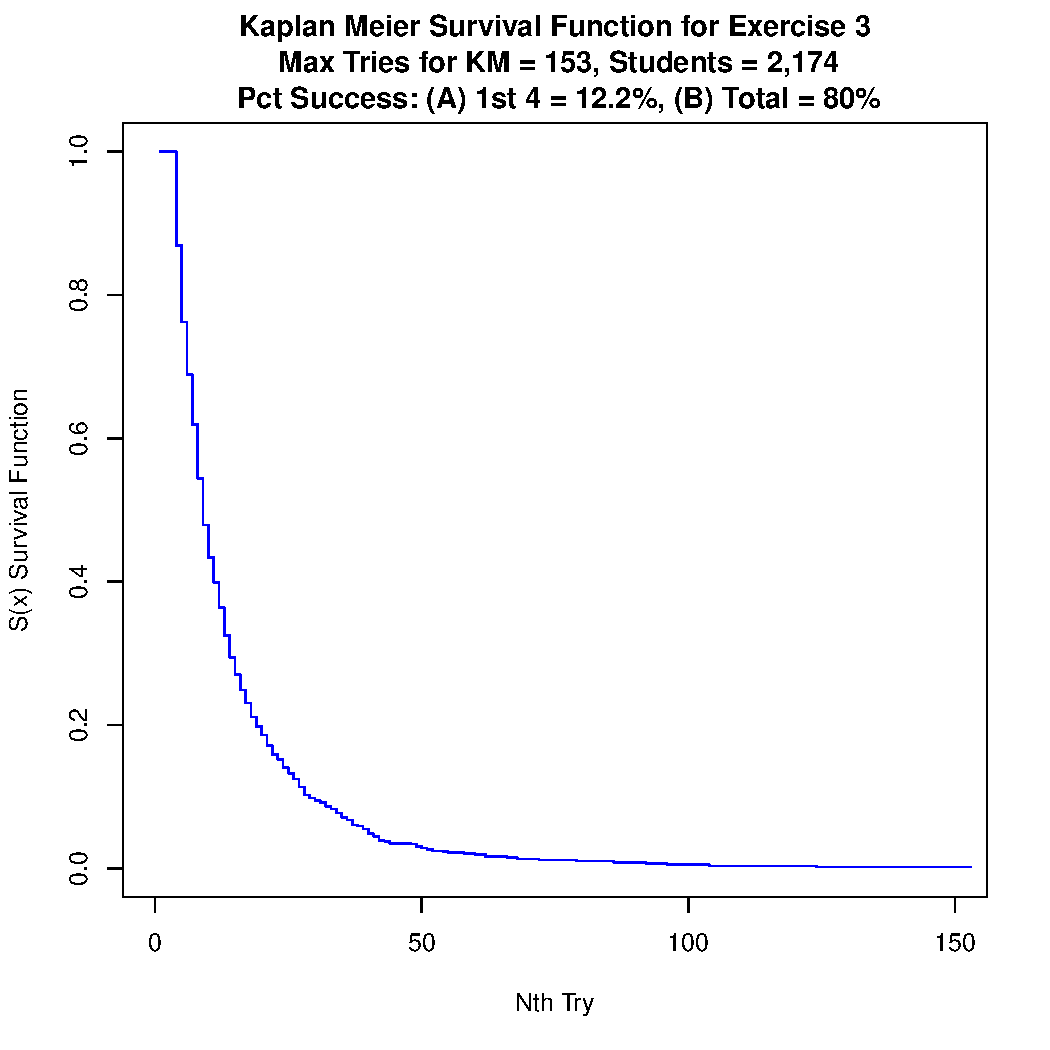
\includegraphics[height=0.9\textheight]{kaplan-meier-1.pdf}
\end{center}
\end{frame}

\begin{frame}[nofills]
\begin{center}
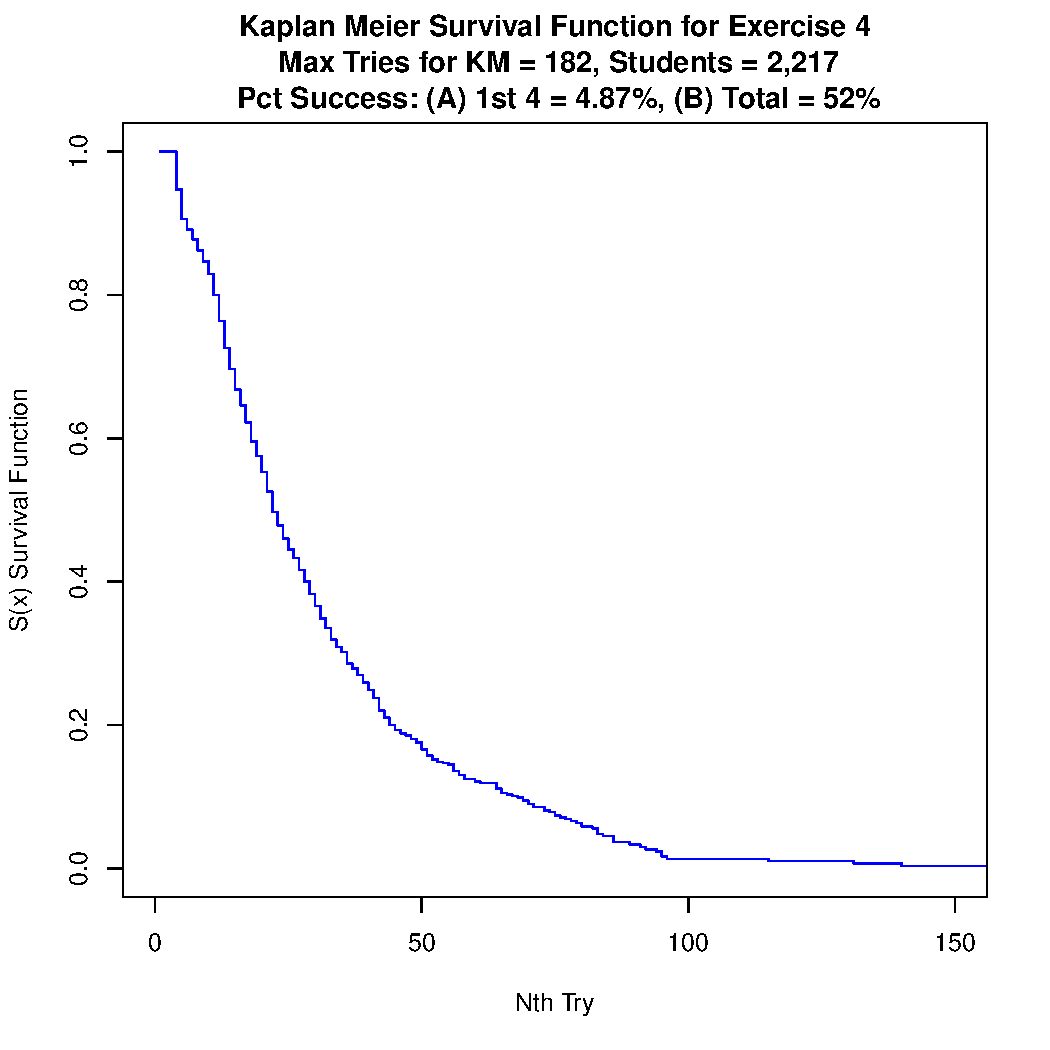
\includegraphics[height=0.9\textheight]{kaplan-meier-2.pdf}
\end{center}
\end{frame}

\begin{frame}[nofills]
\vfill
\huge
point plotting \hfill 91\% correct \\
trig derivatives \hfill 57\% correct \\
related rates \hfill 35\% correct \\
\vfill
\end{frame}


\clearbackgroundpicture
%%%%%%%%%%%%%%%%%%%%%%%%%%%%%%%%%%%%%%%%%%%%%%%%%%%%%%%%%%%%%%%%
\begin{frame}
  \Large

  \textbf{NSF TUES Grant} \\
  \quad for ``Interactive Textbooks''

  \vfill\pause

  Joint with Herb Clemens

  \vfill\pause

  Open source platform for\\
  \quad building open source, \\
  \quad interactive textbooks.

\end{frame}

\setbackgroundpicturewhite{github/mooculus.png}
\begin{frame}
\end{frame}

\setdarkbackgroundpicturewhite{github/mooculus.png}
\begin{frame}[nofills]
\vfill
\huge\textsf{\textbf{Version controlled repository}}
\pause
\vfill
\large\texttt{https://github.com/ASCTech/mooculus}
\vfill
\vfill
\end{frame}

\setbackgroundpicturewhite{github/textbook-sample.png}
\begin{frame}
\end{frame}

\setdarkbackgroundpicturewhite{github/textbook-sample.png}
\begin{frame}[nofills]
\vfill
\huge\textsf{\textbf{Anybody can edit the textbook}}
\vfill
\end{frame}

\setbackgroundpicturewhite{github/commits.png}
\begin{frame}
\end{frame}

\setdarkbackgroundpicturewhite{github/commits.png}
\begin{frame}[nofills]
\vfill
\huge\textsf{\textbf{Complete history of changes}}
\vfill
\end{frame}

\setbackgroundpicturewhite{github/contribution.png}
\begin{frame}
\end{frame}

\setdarkbackgroundpicturewhite{github/contribution.png}
\begin{frame}[nofills]
\vfill
\huge\textsf{\textbf{Students make edits}}
\pause 
\huge\textsf{\textbf{cMOOC meets xMOOC}}
\vfill
\end{frame}

\setbackgroundpicturewhite{github/sequences-and-series.png}
\begin{frame}
\end{frame}


 %%%%%%%%%%%%%%%%%%%%%%%%%%%%%%%%%%%%%%%%%%%%%%%%%%%%%%%%%%%%%%%%
 \clearbackgroundpicture
 \begin{frame}[nofills]
   \vfill
   \begin{center}
   \Huge
    \scalebox{1.5}{\textbf{Thank You}}
   \end{center}
   \vfill
   
\includegraphics[width=1in]{cc-logo.pdf}
   \hfill\footnotesize\scalebox{0.9}{licensed for reuse under a Creative Commons BY-NC-ND License}
   \null
 \end{frame}

\end{document}
